\chapter{Validation}\label{chap:validation}

\minitoc

\section{Methodology} \label{sec:validation_methodology}

As a way to validate the stated hypothesis (\textit{cf.} Section \ref{sec:research_problem}), we have acted upon a thorough process that consists of the following phases:

\begin{enumerate}
    \item \textbf{IaC Tools in Cyber Range Construction}: The role of IaC tools in the context of cyber range construction. % Use Cases | Ansible | Docker 
    \item \textbf{Architecture}: Where details on how the scenario construction process was taken into account, as well as insights on the logic followed.% Ansible
    \item \textbf{Custom Scenarios}: From Linux to Windows-based scenarios, details on how they were developed will be presented and how they can be attacked.
    \item \textbf{Imported Scenarios}: The process of importing scenarios from previous CTF competitions and how they managed to fit in the previously developed scenario construction.
    \item \textbf{Scenario Extensibility}: Details on how new scenarios could be developed and the necessary changes to do so.
    \item \textbf{Cloud Deployment}: Insights on how the cloud deployment was taken into account using Microsoft Azure as the cloud provider.
    \item \textbf{User Interface Panel}: Presentation of the UI responsible for managing scenarios' in a sort of a CTF-level style.
\end{enumerate}


\section{IaC Tools in Cyber Range Construction} \label{sec:validation_iac_tools_in_cr_construction}

According to Masek \textit{et al.} \cite{unleashing_full_potential_of_ansible_ref} ``\textit{the goal of the IaC is to provide system administrators with the ability to manage knowledge and experiences of plenty of subsystems from one place instead of the traditional approach where each subsystem has its dedicated administrator}''. As in the case of this article, Ansible was the selected tool to simplify the orchestration and configuration management tasks related to our subject, as it gives the ability to create a set of YAML playbook files containing procedural instructions on how a target machine should be configured. Its flexibility in working both in Linux and Windows machines and how easy it was to deploy configurations were critical aspects for choosing this tool. 

Across the entire development, Docker was the selected tool responsible for provisioning Docker containers. As Ansible works on a client-only topology, the Ansible application does not need to be installed in the containers. Therefore, Ansible is responsible for both the creation and the issuing of commands to these containers, and as a result, we build an enterprise-level network entirely made of Docker containers by simply issuing a command. The entire process is relatively trivial as long as the necessary configuration files are created, as discussed later. The role of IaC here is phenomenal, as the deployment of our network consists of snippets of code used for declaring how our infrastructure should be configured, which is different from the traditional programming concepts we are currently used to.

Lastly, in particular situations, as we will later see, Vagrant was used in order to create Windows-based scenarios. Essentially the setup we built was a Windows Vagrant box running within the Linux Docker container, letting Windows-based types of attacks be successfully explored by the trainee. One question may arise: \textit{Why not use a Windows VM instead of a Vagrant box inside a Docker container?} The issue with this approach is that more storage will be needed if we intend to run several instances of the Windows VM. Instead, the Docker read-only image will stay the same if we use the first-mentioned approach.
Only the container that derives from that same image will change, adding its read-write layer that interacts with the Docker read-only image. As a result, the system uses way less storage. Concerning Windows-based VMs, a similar approach can be taken into account. In scenarios with more than one Windows VM, an optimal solution to reduce resource consumption would be to use a container with a hypervisor installed responsible for monitoring all the present Windows VMs, instead of having one hypervisor per Windows VM. This can be achieved using linked clones in Vagrant in which new VMs only differing in disk images are created using the parent disk image belonging to a master VM. Another key aspect of choosing this setup was consistency. We wanted to create scenarios based on containers and not use a hybrid approach that used containers and VMs separately. With this, we are ready to move into the architectural details of the project.

The engineering process in the combination of these tools and others that will be later discussed allowed us to obtain a set of cybersecurity training scenarios that can be run locally without needing an enormously complex infrastructure. More specifically, the lightweight containerization approach followed during the development allowed us to run complex scenarios with a distance of a command or click. In Chapter \textbf{CLOUD DEPLOYMENT}, we also discuss how we could export our set of cyber ranges into a remote machine again, with the help of Ansible, to perform every needed remote configuration.

\section{Architecture} \label{sec:validation_architecture}

The scenario construction process using Docker containers targeted enterprise-level networks. As such, corporate environments normally subdivide networks into three different main sections:

\begin{itemize}
    \item \textbf{External Network} refers to the public internet where machines are not controlled by the organization. As such, risk modeling activities should be taken into account in order to evaluate the risk and the probability specific threats and attack scenarios pose to the internals of the organization. With this, according to the organization's budget, decisions on which security measures to place in the company's network are considered and may include systems like Intrusion Detection Systems (IDS), Intrusion Prevention Systems (IPS), Firewalls, Antivirus, among others.
    \item \textbf{Internal Network} which contains the protected machines of an organization, such as internal databases and services only available to the company's employees and not to the general public.
    \item \textbf{Demilitarized Zone (DMZ)}, which is a network that protects the company's internal network and is targeted with untrustworthy traffic. It includes services available to the public and sits between the \textit{External Network} and the \textit{Internal Network}. It generally includes web servers, Domain Name System (DNS) servers, among others.
\end{itemize}

Our project focuses on these three distinct types of networks and considers several network services that we would typically see on enterprise networks, as depicted in Fig. \ref{fig:template_net}

The network architecture presented in Fig. \ref{fig:template_net} shows the services available on every Linux scenario, except for Windows-based scenarios, which slightly differ from this schema. As shown, Ansible appears as the tool responsible for configuring and provisioning the entire network.

\begin{figure}[H]
    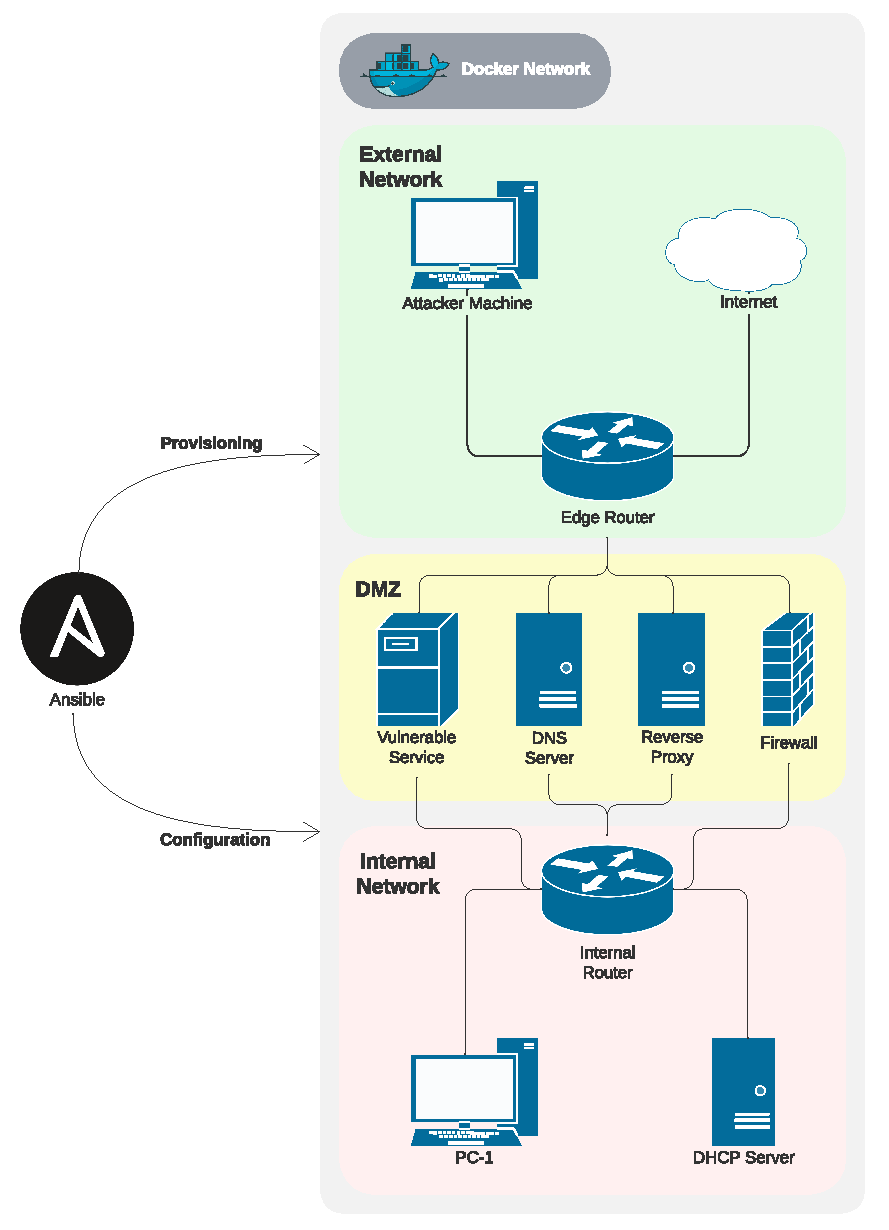
\includegraphics[width=12cm]{figures/example.pdf}
    \caption{Template Network Architecture.}
    \label{fig:template_net}
\end{figure}

\subsection{Ansible Architecture} \label{sec:ansible_structure}

Three different playbooks include all the developed scenarios. The first is explicitly used in Linux-based scenarios, representing most designed challenges. The second is used for the Windows Ransomware scenario, and the last for the Windows Active Directory (AD) scenario. On each one of these playbooks, the first step is always to delete stale Docker containers from previous running scenario executions, as shown in Listing \ref{lst:ansible_removal_of_stale_containers}.

\begin{lstlisting}[language=yaml,caption=Removal of Stale Containers.,numbers=none,label={lst:ansible_removal_of_stale_containers}]
- hosts: localhost
  pre_tasks:
    - name: Remove Stale Containers
      ansible.builtin.include_tasks: teardown.yml
      loop: "{{ machines + vulnerables.machines }}"
      loop_control:
        loop_var: pc_info
\end{lstlisting}

Essentially, for every machine object passed, the contents of the \textit{teardown.yml} file are run. This uses the \textit{community.docker.docker\_container} module that is builtin in Ansible and removes the container under a given name.

\begin{lstlisting}[language=yaml,caption=File \textit{teardown.yml}.,numbers=none,label={lst:ansible_teardown}]
- name: Remove Stale Containers (name="{{ pc_info.name }}")
  community.docker.docker_container:
    name: "{{ pc_info.name }}"
    state: absent
\end{lstlisting}

\subsubsection{Ansible Groups and Inventory} \label{sec:ansible_groups_inventory}

% Inventory & Groups

Every machine belongs to a group, by default in Ansible, the \textit{all} group. Nonetheless, other groups and respective members were defined in the so-called Ansible Inventory, as presented in Listing \ref{lst:ansible_inventory}.

\begin{lstlisting}[caption=High-level view of Ansible Inventory.,numbers=none,label={lst:ansible_inventory},literate={=}{$\rightarrow{}$}{1}]
[routers]
[firewalls]
[external]
[internal]
    = [pcs]
    = [dhcp_servers]
[dmz]
    = [dns_servers]
    = [custom_machines] # Scenario's vulnerable machines.
    = [reverse_proxies]
\end{lstlisting}

As depicted in Listing \ref{lst:ansible_inventory}, each word represents a group of one or more machines. Each group may have several child groups defined by their name, as it happens above, or by machines, represented by their FQDN or IP address. We found groups themselves very useful when restricting certain tasks per group. Then, some groups contain child groups, as happens with the \textit{internal} and \textit{dmz} groups. In the case of Windows-based scenarios, another group called \textit{machine} is used and refers to the Docker container containing the Windows Vagrant box. Listing \ref{lst:ansible_inventory} was a very high-level view of how groups are organized within the project. A custom python inventory script was created to allow the specification of variables across each group.

\subsubsection{Generic Scenario Variables} \label{sec:generic_scenario_variables}

For each playbook, a set of variables are always defined corresponding to the generic structure of the network, as presented in Fig. \ref{fig:template_net}. We start with the Docker images used across the workflow, their path, and the default image name in case none is specified.

\begin{lstlisting}[language=yaml,caption=Ansible Variables - Docker Images.,numbers=none,label={lst:ansible_vars_1}]
general:
  images:
    - name: kali_test_img
      path: ./attacker
    - name: base_image
      path: .
  default_container_image_name: base_image
\end{lstlisting}

As shown in Listing \ref{lst:ansible_vars_1}, we use two Docker images: \textit{base\_image} and \textit{kali\_test\_img}. The former is an image derived from \textit{node:lts-alpine} with some extra packages installed. The Alpine distribution was chosen due to its smaller size compared to other images. As a result, the \textit{base\_image} size is around 230MB. The \textit{kali\_test\_img} is an image derived from the official \textit{kalilinux/kali-rolling} Docker image. This image was extended to include the Xfce\footnote{\url{https://www.xfce.org/}} desktop environment, characterized by its low resource consumption and user-friendliness, as well as \textit{Virtual Network Computing} (VNC) package, which allows screen sharing and remote control from another device, meaning the computer screen, keyboard, and mouse are mapped from an external device to the device installed with VNC. Accessing port 6080 on the target machine makes it possible to obtain remote control over it, which will be later used in the scenarios. This Kali Linux image is especially suited for offensive tasks, and here the only concern was providing the trainee with a broad range of tools he could use in a scenario. Therefore, the image's size is much larger (around 11GB) compared to the \textit{base\_image} used for common network services.

The second category of Ansible variables for machines belonging to the \textit{all} group can be seen in Listing \ref{lst:ansible_vars_2}.

\begin{lstlisting}[language=yaml,caption=Ansible Variables - Docker Networks.,numbers=none,label={lst:ansible_vars_2}]
networks:
  internal_net:
    network_addr: 172.{{ random_byte }}.0.0/24
    gateway_addr: 172.{{ random_byte }}.0.254
    random_byte: "{{ random_byte }}"

  dmz_net:
    network_addr: 172.{{ random_byte | int - 5 }}.0.0/24
    gateway_addr: 172.{{ random_byte | int - 5 }}.0.254
    random_byte: "{{ random_byte | int - 5 }}"

  external_net:
    network_addr: 172.{{ random_byte | int - 10 }}.0.0/24
    gateway_addr: 172.{{ random_byte | int - 10 }}.0.254
    random_byte: "{{ random_byte | int - 10 }}"
\end{lstlisting}

This section concerns Docker networks, according to the structure mentioned in Section \ref{sec:validation_architecture}. The range of each network is defined, as well as the gateway address which points to the host machine. This is mandatory by Docker, as the host machine should always take part in each created virtual Docker network so it can forward packets from and to it later. At last, the \textit{random\_byte} points to a random byte that changes across each scenario execution and confers some degree of randomization as for each new scenario execution, the network IP addresses will change. 

\begin{lstlisting}[language=yaml,caption=Ansible Variables - Machines.,numbers=none,label={lst:ansible_vars_3}]
machines:
  - name: attackermachine
    image: kali_test_img
    volumes:
      - "/dev/net/tun:/dev/net/tun"
    group:
      - external
      - mesh
    published_ports: # There is also the exposed_ports when no mapping to the host machine is needed 
      - 5900:5900
      - 6080:6080
    dns: 
      name: edge_router
      network: external_net
    networks:
      - name: external_net
        ipv4_address: 172.{{ networks.external_net.random_byte }}.0.2
\end{lstlisting}

Listing \ref{lst:ansible_vars_3} presents a typical example of the attacker machine used for offensive tasks. Several attributes are specified according to the logic of a Docker container. We start by its name, the Docker image it uses, possible volumes (anonymous, named, or bind mounts), the groups the container belongs to, and published ports, meaning ports mapped between the Docker container and the host machine. Then, we specify the networks the container belongs to, which can be several, for instance, routers, and lastly, we specify where to find the DNS server. In this case, as the attacker machine is located in the external network, we redirect DNS queries to the edge router's network interface sitting in the external network so that these queries are later forwarded to the DNS server in the DMZ. This is achieved using \textit{iptables} rules. For machines located inside the corporate network, DNS queries are sent directly to the DNS server sitting in the DMZ network without the need for any type of forwarding by the edge router. It is also important to mention other attributes that are also possible to be specified, namely the \textit{devices} and \textit{privilege} attributes. Although Listing \ref{lst:ansible_vars_3} provided only an example of the attacker machine, other network services follow a similar logic.

\subsubsection{Custom Scenario Variables} \label{sec:custom_scenario_variables}

After presenting how the standard setup for each scenario is organized, Listing \ref{lst:ansible_vars_4} shows how customized variables for each scenario are structured, starting with an example of a DNS configuration.

\begin{lstlisting}[language=yaml,caption=Ansible Variables - DNS.,numbers=none,label={lst:ansible_vars_4}]
dns:
  - domain: example-domain.ui.com
    internal:
      machine: vuln_service
      network: dmz_net
    external:
      machine: edge_router
      network: external_net
\end{lstlisting}

Here, a domain named \textit{example-domain.ui.com} is presented along with \textit{internal} and \textit{external} specifications of it. This, as will later be explained, is related to two distinct DNS views that are defined. By ``internal view'' we refer to devices in the internal or DMZ networks; otherwise, they belong to the ``external view''. So, in the listing mentioned above, the \textit{example-domain.ui.com} domain points to the \textit{vuln\_service} container located in the DMZ whenever devices in the ``internal view'' look for this domain. Devices in the ``external view'' point to the external network interface of the edge router. This means resolved DNS requests made by external machines will go through the edge router and be forwarded to the respective machine. 

After talking about DNS, we will go over another set of variables, namely the set of custom machines.

\begin{lstlisting}[language=yaml,caption=Ansible Variables - Custom Images.,numbers=none,label={lst:ansible_vars_5}]
vulnerables:
  images:
    - name: unifi_log4j
      path: scenarios/log4j
      dockerfile: Dockerfile.alpine.mongo
      args:
        VERSION: "6.4.54"
\end{lstlisting}

Listing \ref{lst:ansible_vars_5}, similarly to \ref{lst:ansible_vars_1}, presents the set of Docker images from the collection of custom machines. Still, this representation is a bit more flexible, allowing the specification of the name of the``Dockerfile''' and arguments to be read in the Docker image creation process.

Then, in the vulnerable machines section, the situation is quite the same as in Listing \ref{lst:ansible_vars_3}. The only exception is the variables attribute specific to each machine.

\begin{lstlisting}[language=yaml,caption=Ansible Variables - Custom Machines.,numbers=none,label={lst:ansible_vars_6}]
vulnerables:
  machines:
    - name: reverse_proxy1
      image: reverse_proxy
      # ... #
      vars:
        - domain: adminbot.mc.ax
          targets: 
            - name: admin_bot_frontend
              network: dmz_net
              port: 3000
        - domain: adminbotapi.mc.ax
          targets: 
            - name: admin_bot_api
              network: dmz_net
              port: 8000
\end{lstlisting}

For instance, Listing \ref{lst:ansible_vars_6} refers to an NGINX reverse proxy that redirects requests according to a specified domain. The \textit{vars} attribute specifies which machine and port should be the network packets' target when communicating with a particular domain.

\begin{lstlisting}[language=yaml,caption=Ansible Variables - Port Forwarding.,numbers=none,label={lst:ansible_vars_7}]
port_forwarding:
  - destination_port: 443
    to_machine: reverse_proxy1
    to_network: dmz_net
    to_port: 443
\end{lstlisting}

Then, Listing \ref{lst:ansible_vars_7} references the port forwarding section especially relevant for external machines and how they can communicate with DMZ machines. 

\begin{itemize}
    \item \textit{destination\_port}: the incoming port on the edge router where packets will be redirected.
    \item \textit{to\_machine}: the target machine to which packet reaching the \textit{destination\_port} will be forward to.
    \item \textit{to\_network}: the network where the target machine is placed.
    \item \textit{to\_port}: the destination port in the target machine to where the edge router will redirect packets to.
\end{itemize}

Some names, such as \textit{destination\_port} and \textit{to\_port}, may be misleading. Still, they obey the convention used by \textit{iptables}.

\begin{lstlisting}[language=yaml,caption=Ansible Variables - Setup Section.,numbers=none,label={lst:ansible_vars_8}]
setup:
    machines:
    -   name: localhost
        setup: "{{ playbook_dir }}/scenarios/chessrs/setup/"
    -   name: attackermachine
        setup: "{{ playbook_dir }}/scenarios/chessrs/attacker_machine_setup/*.j2"
\end{lstlisting}

Lastly, we have Listing \ref{lst:ansible_vars_8}, which provides information on where to find the setup instructions for the \textit{localhost} and attacker machines.

\subsubsection{Ansible Roles \& Network Services} \label{sec:ansible_roles}

The structure followed by Ansible used a feature called ``roles''. We used a different role for every milestone in the network configuration. Ansible allows defining specific variables and tasks for each role, making grouping an entire workflow into separate roles straightforward to reuse in the development cycle. The used folder structure can be viewed in Listing \ref{lst:ansible_architecture}.

\begin{lstlisting}[caption=Ansible Roles' Folder Structure.,numbers=none,label={lst:ansible_architecture}]
roles/
    base/             
    custom_machines/
    dhcp/
    dmz/
    dns/
    entrypoint/
    external/
    firewall/
    internal/
    internal_pcs/
    mesh/
    reverse_proxies/
    routers/
\end{lstlisting}

Each directory inside \textit{roles} represents a different role. Inside it, specific tasks are defined.  

\begin{itemize}
    \item \textbf{base}: does 
\end{itemize}